\documentclass[tikz]{standalone}

\usepackage{standalone}

\usepackage{siunitx}

\begin{document}
    \begin{tikzpicture}
        \node[visible on=<2->] (nantes) at (0,0) {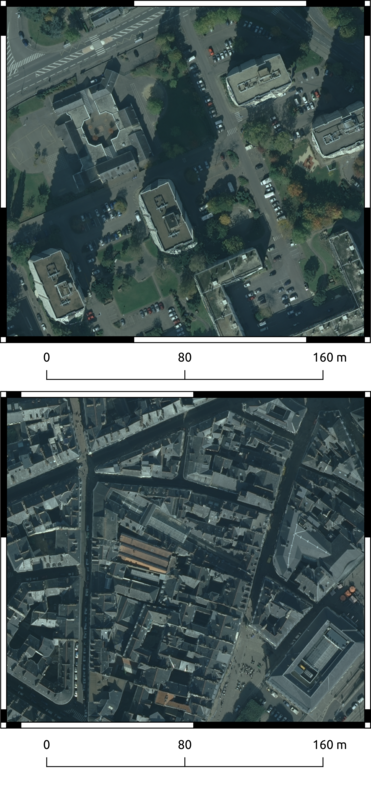
\includegraphics[height=10cm]{images/datasets/nantes_samples}};
        \path (nantes.north) node[anchor=south, text width=4.5cm, align=center, visible on=<2->] (nantes_type) {\large Dense downtown w/. high towers.};
        \path (nantes.south) node[visible on=<2->] (nantes_l) {\large (b) Nantes (\num{748} buildings)};
        \path (nantes_l.south) node[anchor=north, visible on=<2->] {\large Img./DSM res.: \SI{0.1}{\m}};
        \path (nantes.west) + (-1, 0) node[anchor=east] (elancourt) {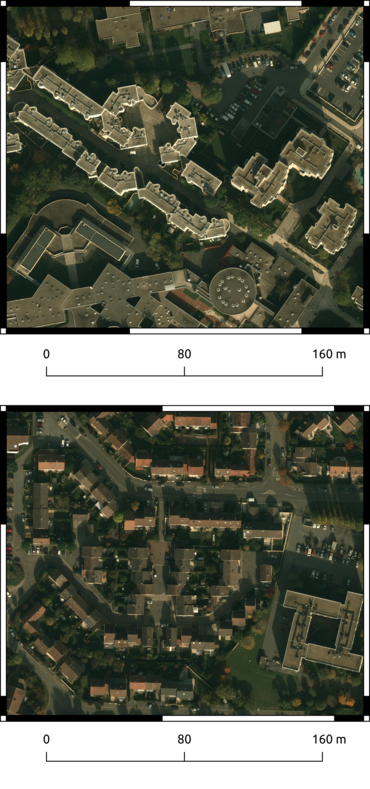
\includegraphics[height=10cm]{images/datasets/elancourt_samples}};
        \path (elancourt.north) node[anchor=south, text width=4.5cm, align=center] (elancourt_type) {\large Industrial \& residential buildings.};
        \path (elancourt.south) node (elancourt_l) {\large (a) Elancourt (\num{2009} buildings)};
        \path (elancourt_l.south) node[anchor=north] {\large Img./DSM res.: \SI{.06}{\m}};
        \path (nantes.east) + (1, 0) node[anchor=west, visible on=<3->] (paris13) {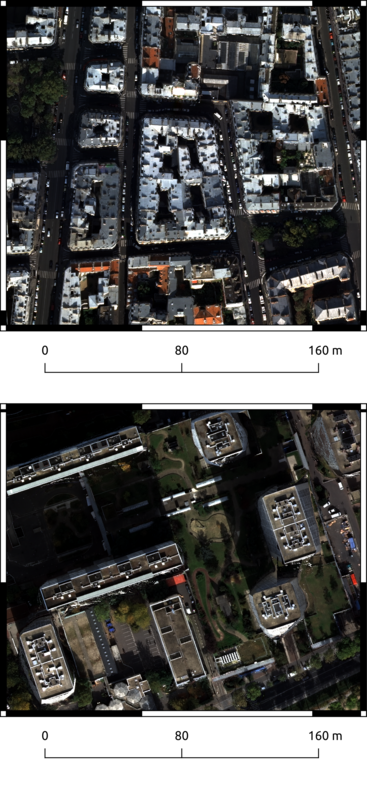
\includegraphics[height=10cm]{images/datasets/paris-13_samples}};
        \path (paris13.north) node[anchor=south, text width=4.5cm, align=center, visible on=<3->] (paris13_type) {\large Hausmann style downtown w/. high towers.};
        \path (paris13.south) node[visible on=<3->] (paris13_l) {\large (c) Paris-13 (\num{478} buildings)};
        \path (paris13_l.south) node[anchor=north, visible on=<3->] {\large Img./DSM res.: \SI{0.1}{\m}};
    \end{tikzpicture}
\end{document}